\documentclass[]{book}

%These tell TeX which packages to use.
\usepackage{array,epsfig}
\usepackage{amsmath}
\usepackage{amsfonts}
\usepackage{amssymb}
\usepackage{amsxtra}
\usepackage{amsthm}
\usepackage{mathrsfs}
\usepackage{color}
\usepackage{graphicx}
\usepackage{float}

%Algorithm packages
\usepackage{algorithm}  
\usepackage{algpseudocode}  
\usepackage{amsmath}  
\renewcommand{\algorithmicrequire}{\textbf{Input:}}  % Use Input in the format of Algorithm  
\renewcommand{\algorithmicensure}{\textbf{Output:}} % Use Output in the format of Algorithm  
%Here I define some theorem styles and shortcut commands for symbols I use often
\theoremstyle{definition}
\newtheorem{defn}{Definition}
\newtheorem{thm}{Theorem}
\newtheorem{cor}{Corollary}
\newtheorem*{rmk}{Remark}
\newtheorem{lem}{Lemma}
\newtheorem*{joke}{Joke}
\newtheorem{ex}{Example}
\newtheorem*{soln}{Solution}
\newtheorem{prop}{Proposition}

\newcommand{\lra}{\longrightarrow}
\newcommand{\ra}{\rightarrow}
\newcommand{\surj}{\twoheadrightarrow}
\newcommand{\graph}{\mathrm{graph}}
\newcommand{\bb}[1]{\mathbb{#1}}
\newcommand{\Z}{\bb{Z}}
\newcommand{\Q}{\bb{Q}}
\newcommand{\R}{\bb{R}}
\newcommand{\C}{\bb{C}}
\newcommand{\N}{\bb{N}}
\newcommand{\M}{\mathbf{M}}
\newcommand{\m}{\mathbf{m}}
\newcommand{\MM}{\mathscr{M}}
\newcommand{\HH}{\mathscr{H}}
\newcommand{\Om}{\Omega}
\newcommand{\Ho}{\in\HH(\Om)}
\newcommand{\bd}{\partial}
\newcommand{\del}{\partial}
\newcommand{\bardel}{\overline\partial}
\newcommand{\textdf}[1]{\textbf{\textsf{#1}}\index{#1}}
\newcommand{\img}{\mathrm{img}}
\newcommand{\ip}[2]{\left\langle{#1},{#2}\right\rangle}
\newcommand{\inter}[1]{\mathrm{int}{#1}}
\newcommand{\exter}[1]{\mathrm{ext}{#1}}
\newcommand{\cl}[1]{\mathrm{cl}{#1}}
\newcommand{\ds}{\displaystyle}
\newcommand{\vol}{\mathrm{vol}}
\newcommand{\cnt}{\mathrm{ct}}
\newcommand{\osc}{\mathrm{osc}}
\newcommand{\LL}{\mathbf{L}}
\newcommand{\UU}{\mathbf{U}}
\newcommand{\support}{\mathrm{support}}
\newcommand{\AND}{\;\wedge\;}
\newcommand{\OR}{\;\vee\;}
\newcommand{\Oset}{\varnothing}
\newcommand{\st}{\ni}
\newcommand{\wh}{\widehat}

%Pagination stuff.
\setlength{\topmargin}{-.3 in}
\setlength{\oddsidemargin}{0in}
\setlength{\evensidemargin}{0in}
\setlength{\textheight}{9.in}
\setlength{\textwidth}{6.5in}
\pagestyle{empty}



\begin{document}


\begin{center}
{\Large COMP 540 \hspace{0.5cm} HW 3}\\
\textbf{Peiguang Wang, Xinran Zhou}\\ %You should put your name here
Due: 1/18/2018 %You should write the date here.
\end{center}

\vspace{0.2 cm}


\subsection*{1: MAP and MLE parameter estimation }

%% Problem 1
\begin{enumerate}
	\item Estimate for $\theta$ using MLE
	\begin{soln}
		The maximum likelihood estimation of $D$ given $\theta$ is that
		$$MLE = l(D|\theta) = p(x^{(i)}) = \prod_{i}^{m} \theta^{x^{(i)}} (1-\theta)^{1-x^{(i)}}$$
		take the NLL of MLE
		$$NLL = -\sum_{i}^{m}[x^{(i)} log \theta +(1-x^{(i)})log (1 - \theta)]$$
		take the derivative of NLL and make it equal to zero
		$$\frac{\partial NLL }{\partial \theta } = -\sum_{i}^{m}[ x^{(i)} \frac{1}{\theta} - \frac{1}{(1-\theta)}(1- x^{(i)})] = 0$$
		by computing this equation, we can get $\theta_{MLE}$
		$$\theta_{MLE} = \frac{1}{m} \sum_{i}^{m} x^{(i)}$$
		
	\end{soln}
	\item Compare the MAP and MLE estimates of $\theta$
	\begin{soln}
		If we add a conjugate prior and use both the D and this prior to make a estimation of $\theta$, we can have this
		\begin{equation*}
			\begin{split}
			MAP &=l(D|\theta)Beta(D|a,b)\\
				&=[\prod_{i}^{m} \theta^{x^{(i)}}(1-\theta)^{1-x^{(i)}}]\theta^{a-1}(1-\theta)^{b -1}
			\end{split}
		\end{equation*}
		take the derivative of $\theta$ and make it equal to zero, we can get $\theta_{MAP}$
		$$\theta_{MAP} = \frac{\sum_{i}^{m}x^{(i) }+ a + 1}{ m + a + b - 2}$$
		if $a = b= 1$ then 
		$$\theta_{MAP} = \theta_{MLE}=\frac{1}{m}\sum_{i}^{m} x^{(i)}$$
	\end{soln}

\end{enumerate}
%%problem 2 
\subsection*{2: Logistic regression and Gaussian Naive Bayes }
\begin{enumerate}
	\item  For logistic regression, what is the posterior probability for each class, i.e.,
	$P (y = 1|x)$ and $P (y = 0|x)$? Write the expression in terms of the parameter $\theta$ and the sigmoid function.
	\begin{soln}
		$$P (y = 1|x) = h_{\theta}(X) = \frac{1}{1+e^{-\theta^T X}}$$
		$$P (y = 0|x) = 1 - h_{\theta}(X) = \frac{e^{-\theta^T X}}{1+e^{-\theta^T X}}$$
	\end{soln}
	\item Derive the posterior probabilities for each class
	\begin{soln}
		The Gaussian distribution and Bernoulli distribution that we assume
		$$ P(y = 1) = \gamma$$
		$$ p (x_j|y = 1) = N(\mu_j^1, \sigma_j^2)$$
		$$P(x_j|; y =0) = N(\mu_j^0, \sigma_j^2)$$
		Naive Bayes model
		$$ p(x|y) = \prod_{j}^{d}P(x_j|y)$$
		Bayes rule
		$$P(y = 1|x) = \frac{P(y=1)P(x|y =1)}{\sum P(y = i)P(x|y =i)}$$
		so these are what we can use now, then we will derive the posterior probabilities
		\begin{equation*}
			\begin{split}
			p(y = 1|x)& = \frac{P(y=1)P(x|y =1)}{ P(y = 0)P(x|y =0)+ P(y = 1)P(x|y =1)}\\
				&= \frac{\gamma \prod_{j =1}^{d} N(\mu_j^1, \sigma_j^2)}{\gamma \prod_{j =1}^{d} N(\mu_j^1, \sigma_j^2) + (1 -\gamma) \prod_{j =1}^{d} N(\mu_j^0, \sigma_j^2)}\\
				&=\frac{1}{1+ \frac{1-\gamma}{\gamma} \prod_{j =1}^{d} exp(\frac{(x_j-\mu_j^1)^2 - (x_j-\mu_j^0)^2}{2\sigma_j^2 })}
			\end{split}			
		\end{equation*}
		the probability $P(y = 0|x)$ can be derived using the same method or just subtract it from 1.
	\end{soln}
	\item part 3
	\begin{soln}
			Class 1 and class 0 are equally likely, that means $\gamma = \frac{1}{2}$
			the probability equation can be written as 
			$$P(y = 1|x) =\frac{1}{1+ \frac{1-\gamma}{\gamma} \prod_{j =1}^{d} exp(\frac{(x_j-\mu_j^1)^2 - (x_j-\mu_j^0)^2}{2\sigma_j^2 })}$$
			if we set $ \mu_j^0 = - \mu_j^1$ then we have
			$$P(y = 1|x) = \frac{1}{1+ \prod_{j =1}^{d} e^(\frac{2 x_j \mu_j^0}{\sigma_j^2})}$$
			obviously it has the same form as logistic regression, if we see in this way
			$$ \theta = [ \frac{2\mu_1^0}{\sigma_1^2}, \frac{2\mu_2^0}{\sigma_2^2},...,\frac{2\mu_d^0}{\sigma_d^2}]^T$$
			$$X = [x_1, x_2,...,x_d]^T$$
			the equation can be rewritten using $\theta$ and X
			$$P(y = 1|x) = \frac{1}{1+e^{-\theta^T X}}$$
		
	\end{soln}
\end{enumerate}
\subsection*{3: Reject option in classifiers  }
\begin{enumerate}
	\item part 1
	\begin{soln}
		The loss of choosing a class j is 
		$$loss = \lambda_s (1 - P(y = j | x))$$
		then if we want to decide $y=j$, we need to make $loss \leq \lambda_r$, which means that
		$$\lambda_s(1 - P(y = j | x))\leq \lambda_r$$
		so
		$$ P(y = j | x)\geq 1- \frac{\lambda_r}{\lambda_s}$$
	\end{soln}
	\item When $\frac{\lambda_r}{\lambda_s}$ approches to 0, the cost of falsely classifying is extremely large,which means that the cost of rejects is small, so we tend to choose rejection.
	As  $\frac{\lambda_r}{\lambda_s}$ increases, the cost of rejection increases. And when $\frac{\lambda_r}{\lambda_s} = 1$ we would never reject.
\end{enumerate}
\subsection*{4: Kernelizing k-nearest neighbors  }
\subsection*{5: Constructing kernels  }
\begin{enumerate}
	\item $k(x,x^{'}) = C k_1(x,x^{'})$
	\begin{soln}
		$$C k_1(x,x^{'}) = C \Phi_1(x)^T \Phi_1(x^{'}) = (\sqrt{C}\Phi_1(x)^T)(\sqrt{C}\Phi_1(x^{'})^T)$$
		if $C\geq0$ then $k(x,x^{'})$ is a valid kernel.
	\end{soln}
	\item $k(x,x^{'}) = f(x) k_1(x,x^{'}) f(x^{'})$
	\begin{soln}
		$$f(x) k_1(x,x^{'})f(x^{'}) = <f(x)\Phi_1(x),  f(x^{'})\Phi_1(x^{'})>$$
		since it satisfy the Mercer's theorem, $k(x,x^{'})$ is valid
	\end{soln} 
	\item $(x,x^{'}) = k_1(x,x^{'}) + k_1(x,x^{'})$
	\begin{soln}
		Because $k_1(x,x^{'}$ and $k_2(x,x^{'}$ both are valid kernels, so by Mercer's theorem they both satisfy
		$$\int_d k(x,x^{'})f(x)f(x^{'})\geq0$$
		then $k(x,x^{'}) = \Phi(x)^T \Phi(x^{'})$ exists.
		So 
		$$k_1(x,x^{'} + k_2(x,x^{'}) = \int_d k_1(x,x^{'}f(x)f(x^{'})) + \int_d k_2(x,x^{'}f(x)f(x^{'}))$$
		Because $\int_d k_1(x,x^{'}f(x)f(x^{'})) > 0 $ and $\int_d k_2(x,x^{'}f(x)f(x^{'})) > 0 $, so
		$$k_1(x,x^{'} + k_2(x,x^{'}) \ge 0$$
	\end{soln}
\end{enumerate}
\subsection*{6: One vs all logistic regression  }
\begin{enumerate}
	\item Implementing and predicting a one-vs-all classifier for the CIFAR-10 dataset.
	
	\begin{figure}[H]
		\centering
		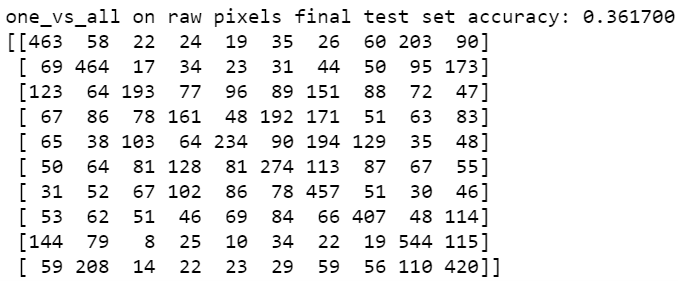
\includegraphics[width=8cm]{ova.png}
		\caption{confusion matrix of ova}
		\label{fig:1}
	\end{figure}
	\item Visualizing the learned parameter matrix
	
	\begin{figure}[H]
		\centering
		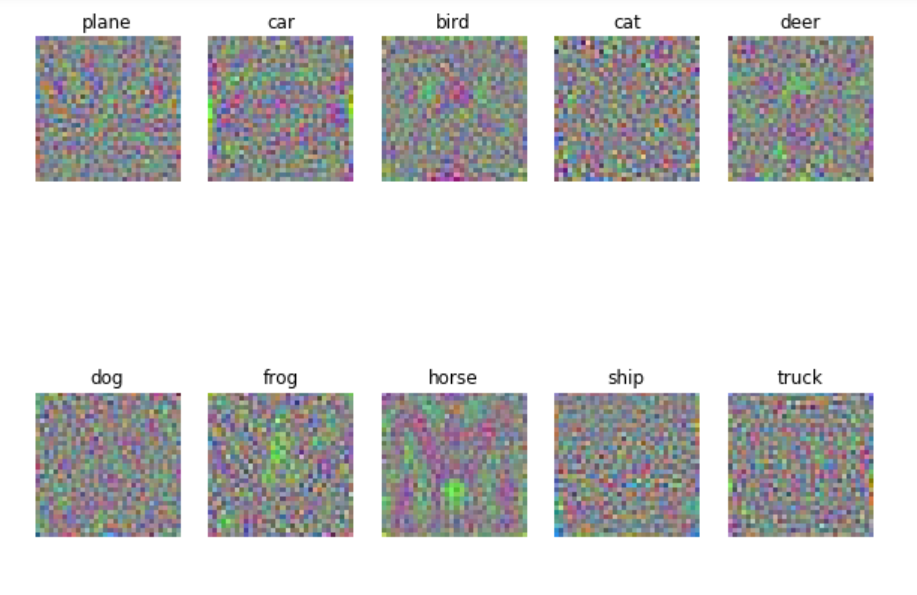
\includegraphics[width=8cm]{ova_1.png}
		\caption{learned one-vs-all classifier visualization}
		\label{fig:2}
	\end{figure}
	\begin{figure}[H]
		\centering
		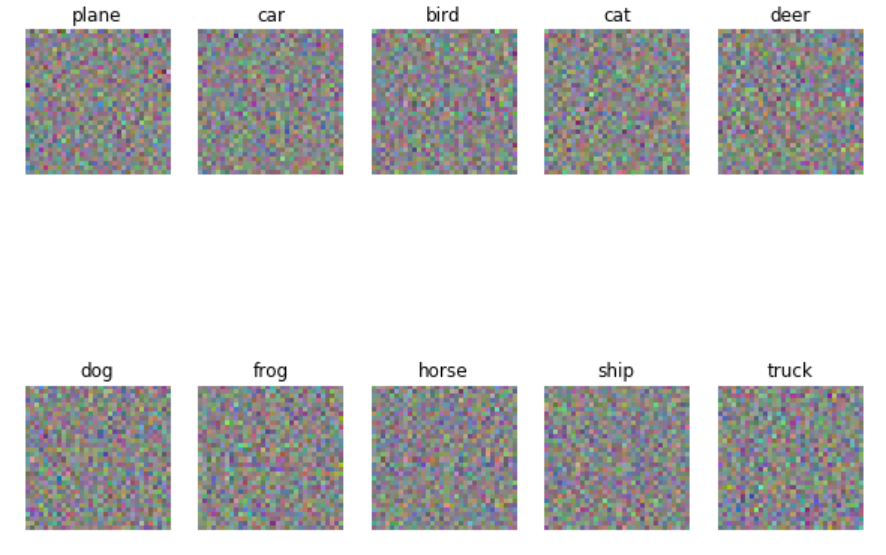
\includegraphics[width=8cm]{ova_2.png}
		\caption{sklearn OVA classifier visualization}
		\label{fig:3}
	\end{figure}
	
\end{enumerate}
\subsection*{7: Softmax Regression}
\begin{enumerate}
\item loss function for softmax regression (naive version)
\begin{soln}
	When implemented in naive version, the softmax regression results are shown in below. Note it took 14.744 seconds to compute the loss. \\
	\textsl{numerical: -3.709464 analytic: -3.709464, relative error: 8.806310e-09 \\
	numerical: -0.474544 analytic: -0.474544, relative error: 5.447825e-08 \\
	numerical: 2.137769 analytic: 2.137769, relative error: 1.418326e-08 \\
	numerical: 2.231634 analytic: 2.231634, relative error: 5.038103e-08 \\
	numerical: 0.342416 analytic: 0.342416, relative error: 3.329287e-08 \\
	numerical: 2.323395 analytic: 2.323395, relative error: 1.629854e-08 \\
	numerical: -0.570532 analytic: -0.570532, relative error: 2.058362e-08 \\
	numerical: 1.082908 analytic: 1.082908, relative error: 5.096985e-10 \\
	numerical: 0.440409 analytic: 0.440409, relative error: 3.809953e-08 \\
	numerical: 2.232702 analytic: 2.232702, relative error: 2.706612e-08 \\
	naive loss: 2.352202e+00 computed in 14.744000s}
\end{soln}
\item loss function for softmax regression (vectorized version)
\begin{soln}
	When implemented in naive version, the softmax regression results are shown in below. Note it took 0.483000 seconds to compute the loss. \\
	\textsl{
	vectorized loss: 2.352202e+00 computed in 0.483000s \\
	Loss difference: 0.000000 \\
	Gradient difference: 0.000000}
\end{soln}
\item Compare naive version and vectorized version

\begin{soln}
	It took 14.744000s for naive version to compute the result; and 0.483000 for vectorized version. The vectorized version is much faster than the naive version.
\end{soln}

\item Using a validation set to select regularization lambda and learning rate for gradient descent.
\begin{soln}
	We choose mini patch size 400, and set the number of iteration to 4000. The program result is:\textsl{Best validation accuracy achieved during cross-validation: 0.418000}
\end{soln}

\item Evaluating the best softmax classifier on the test set and visualizing the coefficients
\begin{soln}
	Using the selected best softmax model on testing dataset. The program result is:
	
	\textsl{softmax on raw pixels final test set accuracy: 0.405100 }
	
	Visualize the coefficients in Figure \ref{fig:cofficient}.  
	\begin{figure}[H]
		\centering
		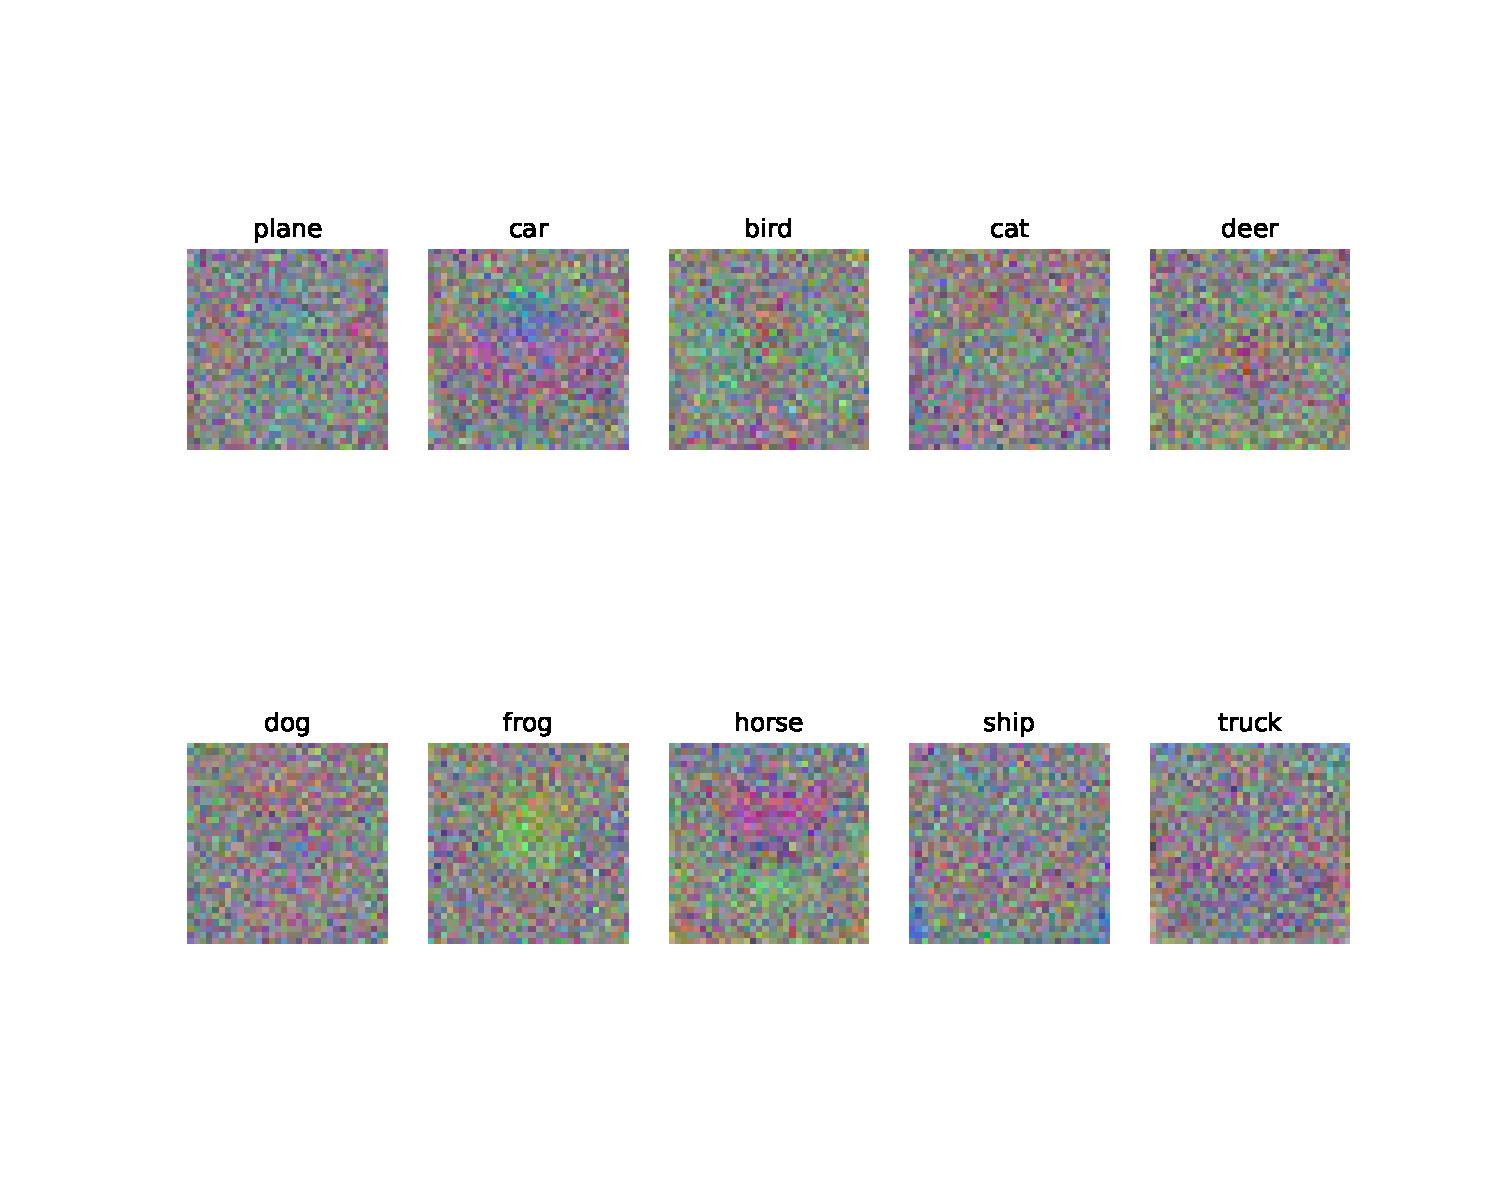
\includegraphics[width=10cm]{cofficients.pdf}
		\caption{Visualization of the cofficients}
		\label{fig:cofficient}
	\end{figure}

\end{soln}

\end{enumerate}


\end{document}


